\providecommand{\relativeRoot}{../..}
\documentclass[\relativeRoot/main.tex]{subfiles}
\graphicspath{{\subfix{./figures/}}}


\begin{document}

\section{Implementation}
\label{sec:lyprox:implementation}

\subsection*{Database Models}
\label{subsec:lyprox:implementation:models}

\begin{figure}
    \centering
    \def\svgwidth{1.0\textwidth}
    \input{figures/er_diagram_paths.pdf_tex}
    \caption[
        ER diagram of LyProX' data model
    ]{
        \Acrlong{er} diagram of LyProX' underlying data representation. Every box corresponds to one Python \texttt{class} in Django and therefore also to one table in the SQLite3 database. Entries in those tables are linked to other table's entries via the indicated connections. The connections between nodes of this graph are all \emph{one-to-many} relations, meaning that e.g. one institution per user, but many users per institution.
    }
    \label{fig:lyprox:er_diagram}
\end{figure}

The first step in creating a Django web application -- aside from initializing the project by choosing important settings -- usually consists of defining the database models. This is done by writing a Python class that inherits from Django's \texttt{Model} class for each type of object one wants to store. One such class essentially corresponds to a table in the underlying database (e.g., an \acrshort{sql} database like \href{https://www.sqlite.org/index.html}{SQLite3}). It can be given attributes for each column in that table and may also store relationships between tables/classes. Based on this Python representation of data, Django can automatically create extensive functionality. As their documentation states: 

\begin{displayquote}[Django documentation \cite{noauthor_creating_nodate}]
    The goal is to define your data model in one place and automatically derive things from it.
\end{displayquote}

For example, when we defined the \texttt{Patient} class, we used Django to generate large parts of the utilities that render \acrshort{html} forms for creating, editing and deleting \texttt{Patient} entries in the respective SQLite3 database. In total, we created six entities to represent our patient cohorts in the database:

\begin{itemize}
    \item \texttt{Insitution:} Represents a hospital or medical research facility that has created datasets of patients, e.g. from their treatment records.
    \item \texttt{User:} A member of one of the \texttt{Institutions} who uploaded data into the web page's database or whom we granted access to particular \texttt{Datasets} we did not yet make public.
    \item \texttt{Dataset:} Groups \texttt{Patients} into cohorts that were extracted or added to the interface at the same time. This entity stores additional information such as the repository it is made persistent in -- if available -- or whether it is public. \texttt{Datasets} that are not public were implemented to be able to visualize progression patterns of patient cohorts that are not ready for publication yet.
    \item \texttt{Patient:} The core entity in the database corresponding to a patient record. It encodes e.g. demographic information such as age and sex, as well as TNM stage. It belongs to a \texttt{Dataset} and can hold multiple \texttt{Tumors} and \texttt{Diagnoses}.
    \item \texttt{Tumor:} We could have added information about the primary tumor directly to the \texttt{Patients} table, but at some point we might want to be able to deal with multiple synchronous tumors. Due to this potential extension in the future, we created a separate entity for tumors and allow a \texttt{Patient} to be associated with multiple tumors. It stores tumor-specific data, such as its location, lateralization and volume -- if available.
    \item \texttt{Diagnose:} For the reporting of \acrlong{lnl} involvement, this is the Django \texttt{class} of interest. For each side of a \texttt{Patient's} neck (ipsi- and contralateral) and for each modality that reported lymphatic involvement (e.g. \gls{mri}, \gls{ct}, pathology, ...), one such entry exists. It stores whether each \gls{lnl}'s state was reported to be metastatic, healthy or unknown (as is often the case when an \gls{fna} is performed).
\end{itemize}

A detailed \acrlong{er} diagram is shown in \cref{fig:lyprox:er_diagram}. It also lists all attributes that are stores for each entity and what Django type is used to represent them.

\subsection*{Adding Patients Manually}
\label{subsec:lyprox:implementation:add_manual}

\begin{figure}
    \centering
    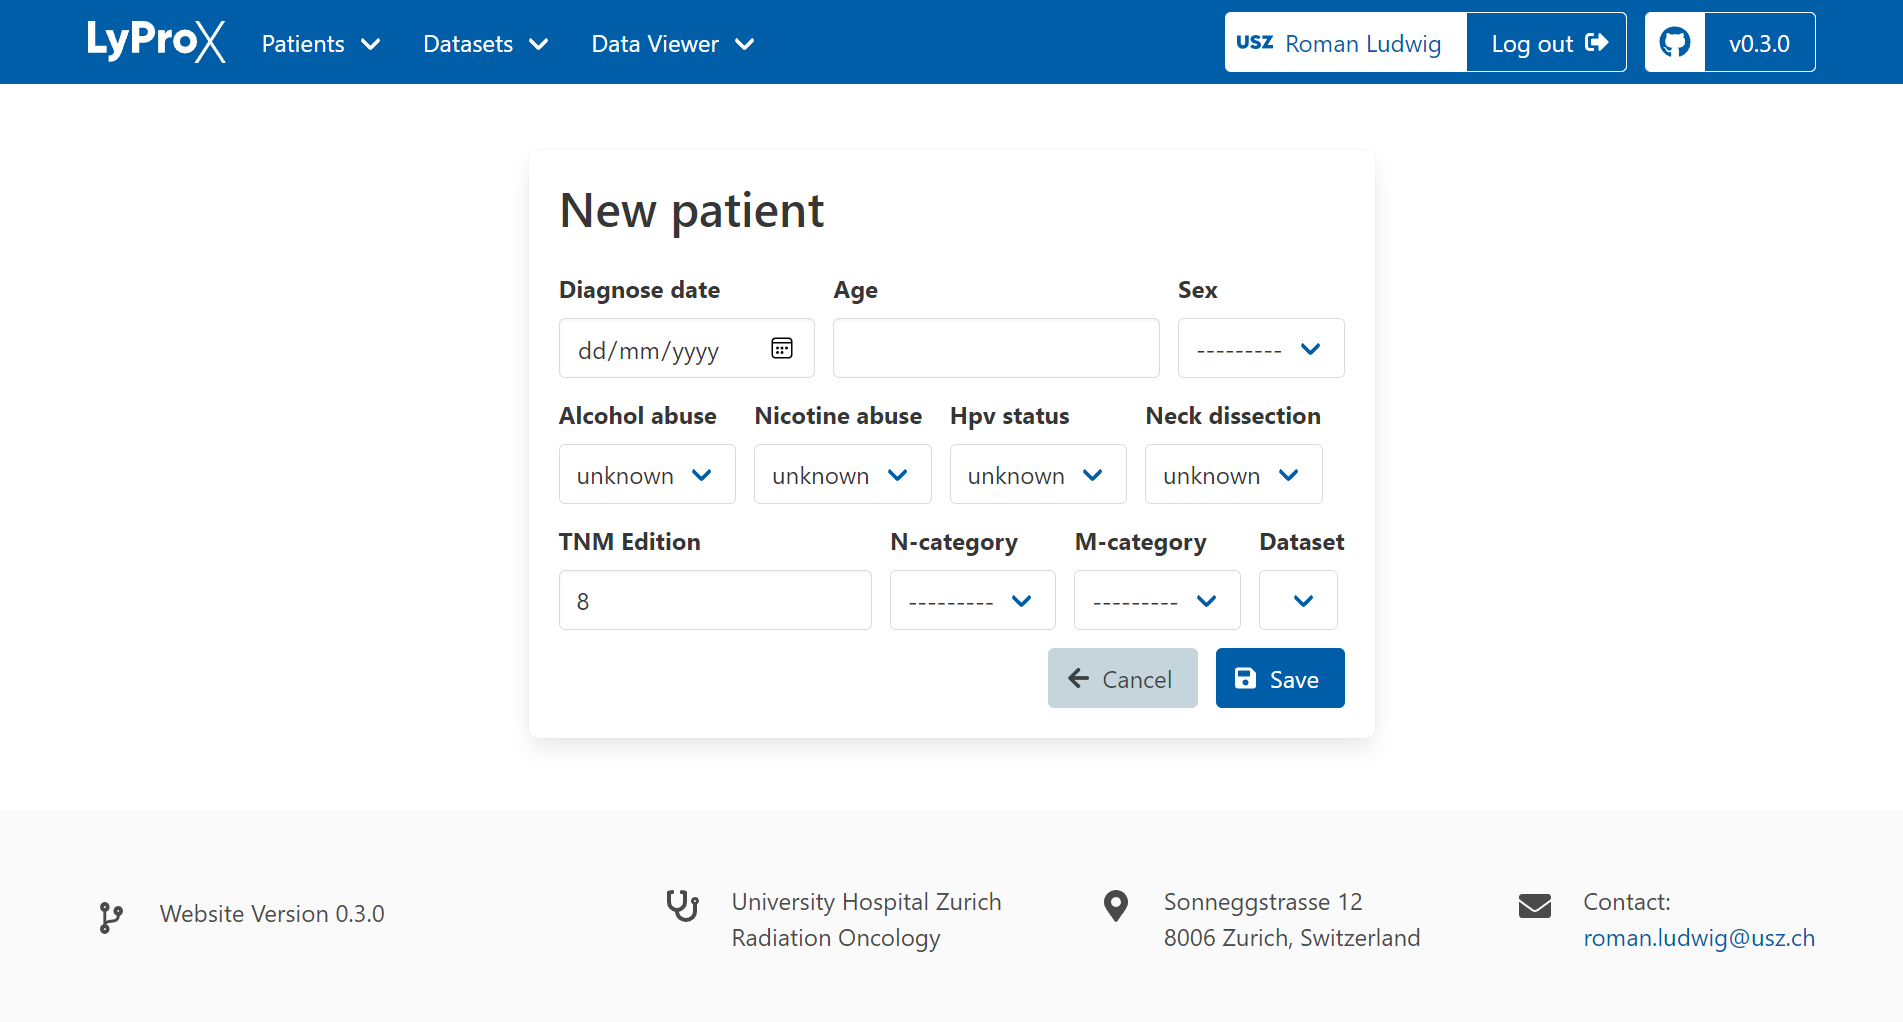
\includegraphics[width=1.0\textwidth, frame]{figures/new_patient.png}
    \caption[
        Screenshot of the form for adding new patients
    ]{
        Screenshot of the rendered \acrshort{html} form that is shown when an authenticated user wants to add a new \texttt{Patient} to an existing \texttt{Dataset}. Note that the form contains no field for specifying a T-category.
    }
    \label{fig:lyprox:new_patient}
\end{figure}

Django's design principles allow developers to reuse as much as possible of already written code. Hence, most of the functionality to add, edit or delete any of the just introduced database entities was already implemented. Django does this via \texttt{Form} classes that are built around the user-created \texttt{Model} classes. Those Django forms can then in turn render \acrshort{html} forms into which a user can enter data that -- when sent back to the server -- will be translated by the same \texttt{Form} class into a new or changed database entry.

On top, one may implement custom logic to sanitize a user's input or derive \texttt{Model} attributes from inputs. An example in LyProX would be the T-category: As shown in \cref{fig:lyprox:er_diagram}, for every \texttt{Patient}, we store the attribute \texttt{t\_stage}. But when creating a new patient (see screenshot in \cref{fig:lyprox:new_patient}), there is no field for T-category. After the new \texttt{Patient} entry has been created, however, one may add a \texttt{Tumor} to it, for which a T-category must be defined. Upon writing the tumor information into the database, Django calls a method in the \texttt{Patient} class updating this instance's T-category to be the most advanced of all its tumors. This can be seen in \cref{fig:lyprox:sanitize_t_stage}, where the patient's T-category is set to 0 initially. Then, a T2 tumor is added to that patient and the patient's T-category immediately updates to be T2 as well.

\begin{figure}
    \centering
    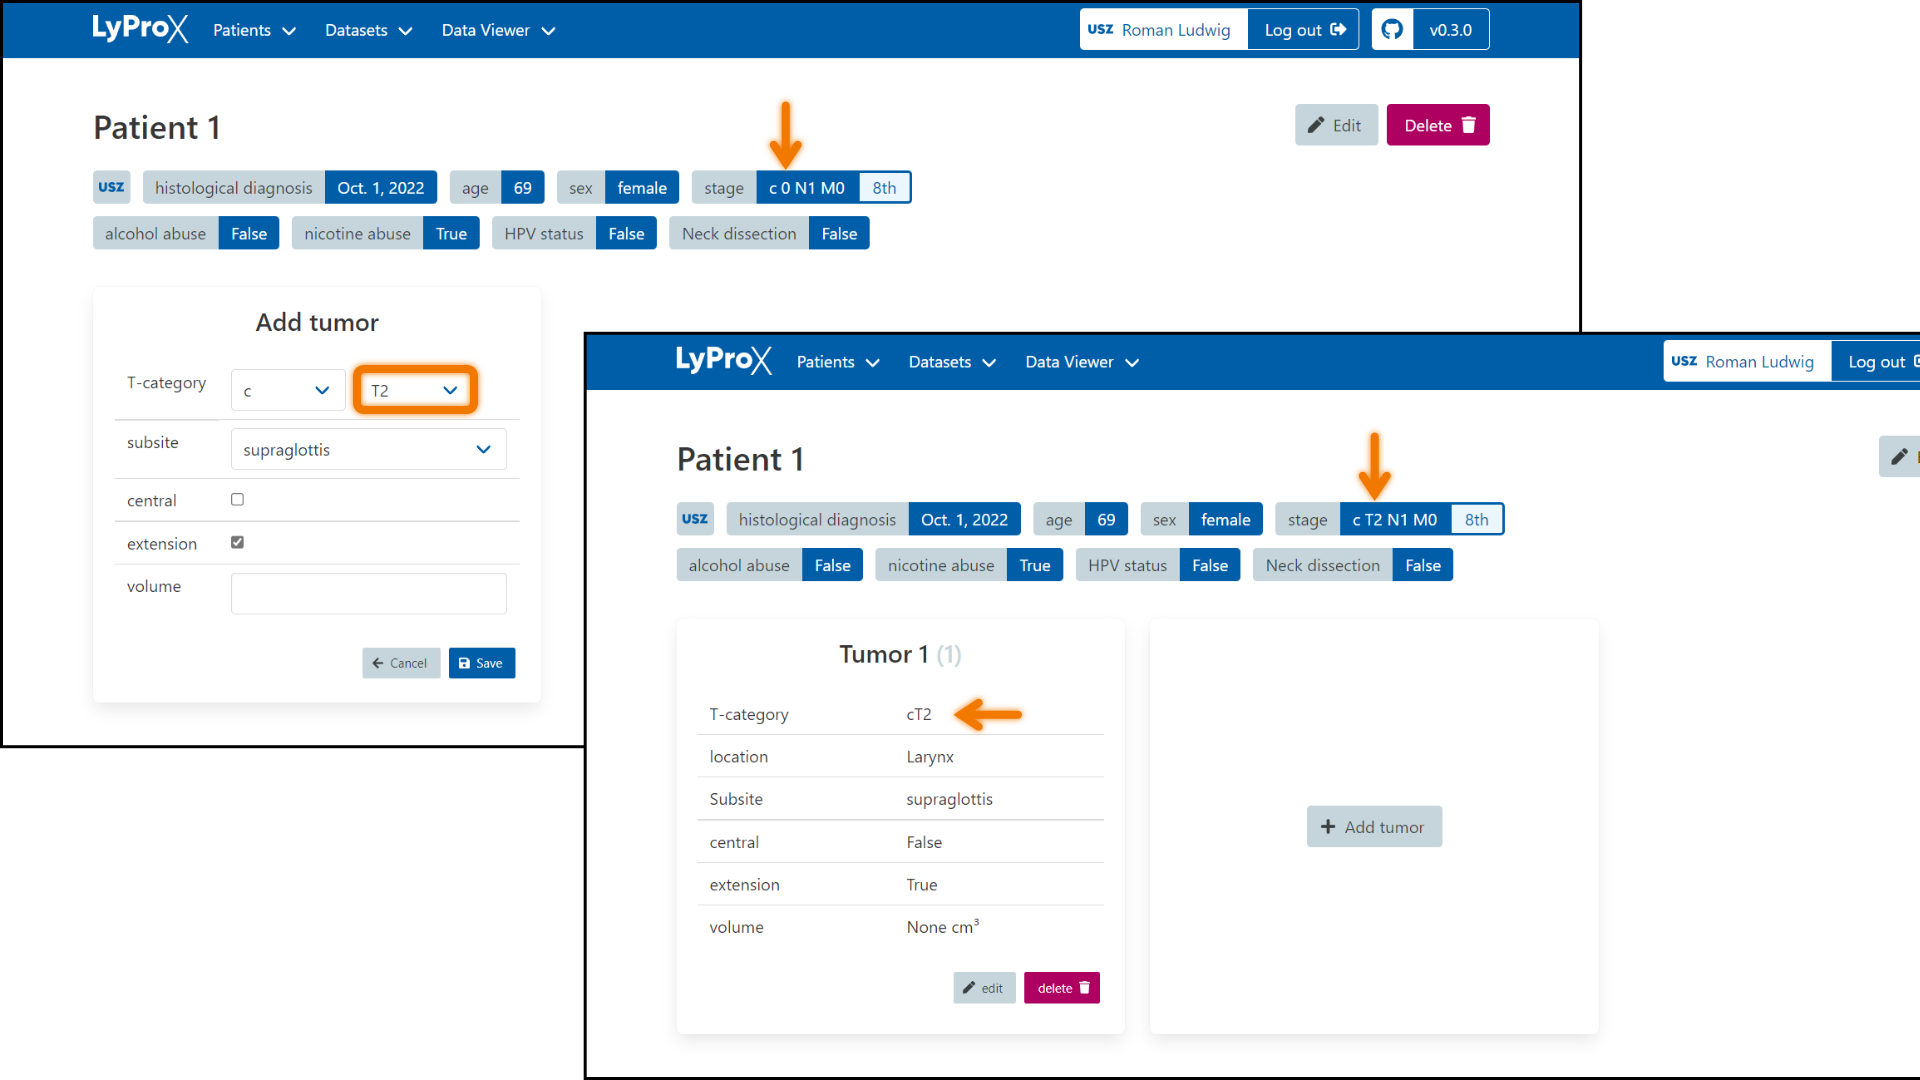
\includegraphics[width=1.0\textwidth]{figures/sanitize_t_stage.png}
    \caption[
        Process of adding a new tumor to a patient
    ]{
        Screenshot of the page displaying the newly created patient where information about the primary tumor is just being filled in (top left panel in the back), as well as a screenshot of the same patient page after the tumor was added (bottom right panel in front). The orange arrows indicate how the information is added during the process.
    }
    \label{fig:lyprox:sanitize_t_stage}
\end{figure}

Similarly, we implemented sanitization of some \glspl{lnl} in the \texttt{Diagnose}, where we need to make sure that the combination of lymphatic super- and sublevels is consistent. E.g., if we add a \texttt{Diagnose} to a \texttt{Patient} and report \gls{lnl} IIa to be healthy, but the other sublevel IIb to harbor metastases, then we automatically set the super level II to ``involved''. The other way around, when \gls{lnl} II is entered as being healthy, we can deduce that all sublevels (IIa and IIb) must be set to healthy, as well.

After adding \texttt{Patient} entries to a \texttt{Dataset}, it can be locked to preserve it as created by preventing accidental edits. A method in the \texttt{Dataset's} definition is called whenever an attempt to change a \texttt{Patient}, \texttt{Tumor} or \texttt{Diagnose} is made, and raises an exception before the change can be written to the SQLite3 database.

\subsection*{Batch-Importing Datasets}
\label{subsec:lyprox:implementation:batch_import}

The data representation of LyProX allows it to be used in the initial stage of data collection by entering patients manually one by one. But we also implemented methods for batch importing previously curated datasets. This means we can take any spreadsheet-like file, rename its column headers according to what LyProX expects and batch-import entire patient cohorts as a \gls{csv} file.

The \gls{csv} format that is expected by LyProX, and documented at \href{https://lyprox.org/dataset}{\faIcon{external-link-alt}~\texttt{https://lyprox.org/dataset}}, is also used in the implementation of the probabilistic \repolink{lymph} model (see also  \cref{chap:unilateral}) to load the data for learning, and for publishing our raw data in \repolink{lyDATA}, where it is described again.

\subsection*{Visualizing Patterns of Progression}
\label{subsec:lyprox:implementation:viewer}

\begin{figure}
    \centering
    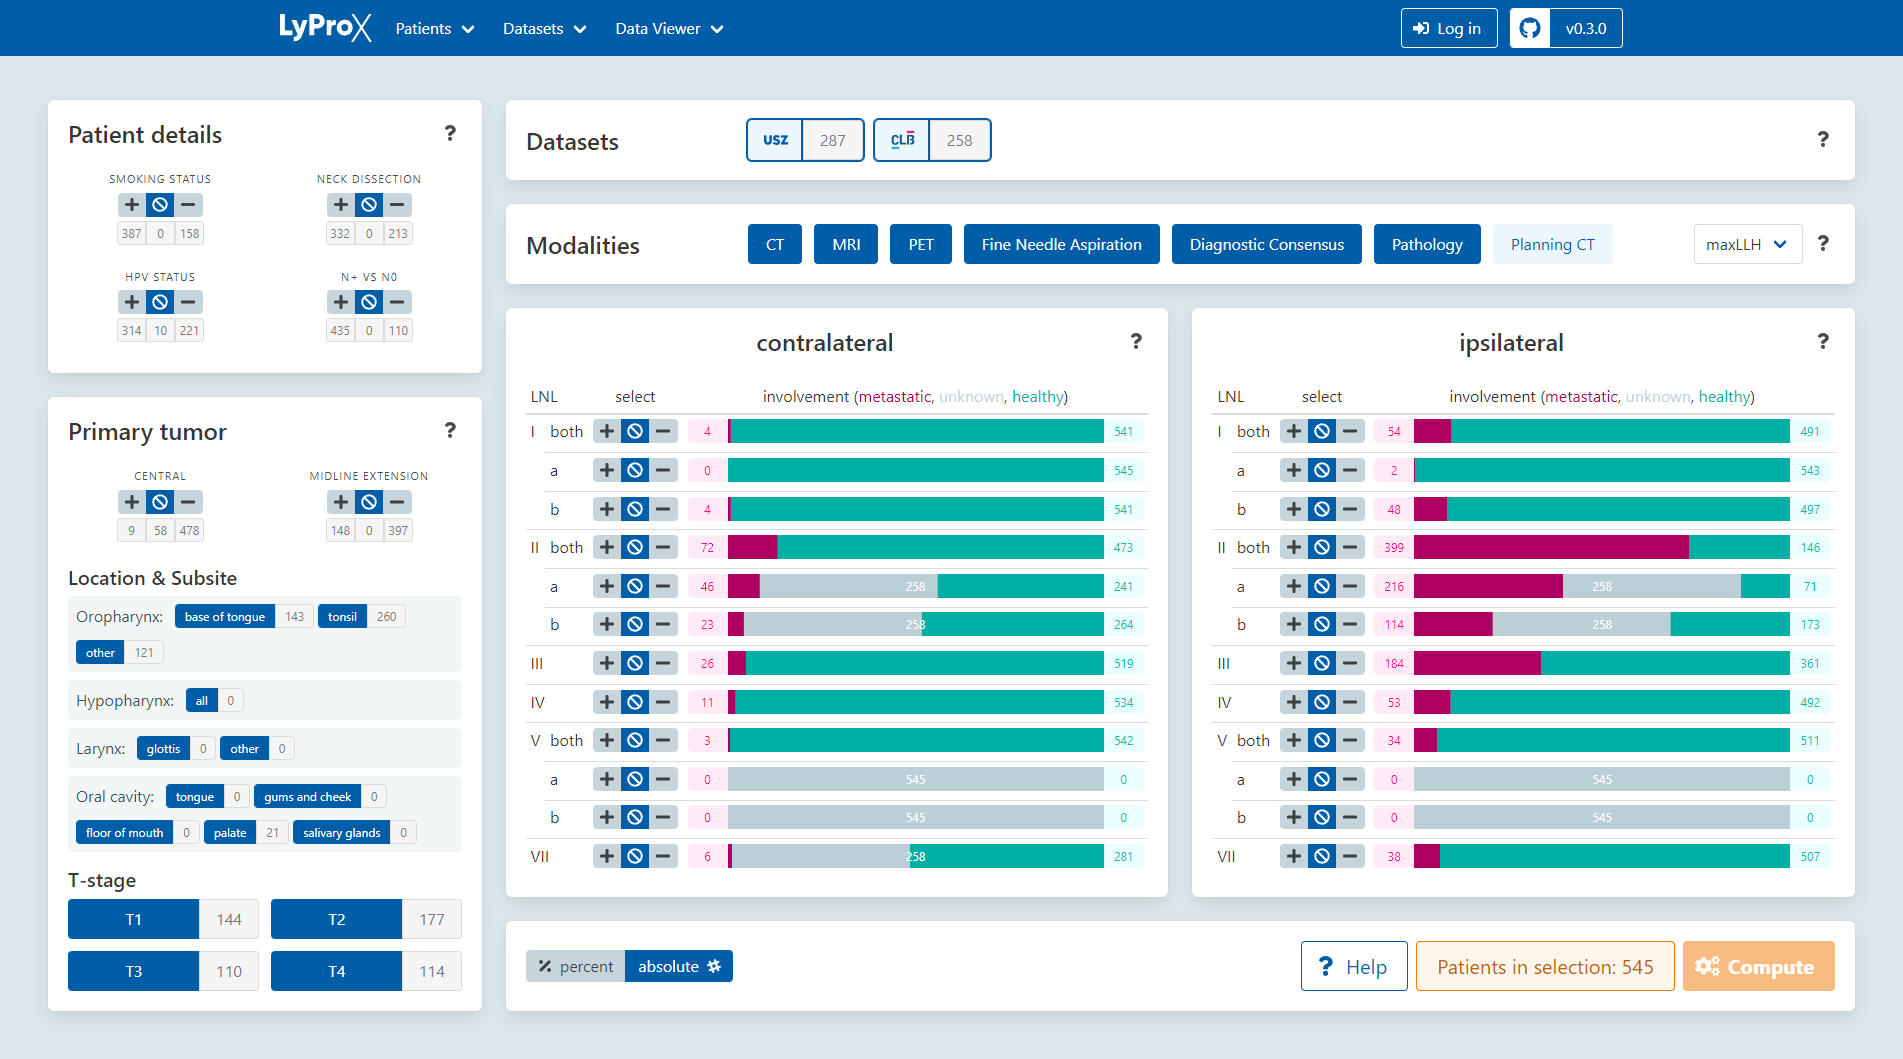
\includegraphics[width=1.0\textwidth, frame]{figures/data_viewer.png}
    \caption[
        Screenshot of the data viewer dashboard
    ]{
        A screenshot of the data viewer. Users can filter patients in the datasets by different criteria: General information, e.g. \gls{hpv} status (top left box), tumor characteristics like location and T-category (bottom left box), dataset of origin (top right bar), which reported modalities to include and how to combine them (second bar from top, right side) and finally they may be filtered by per-level involvement (two tall boxes in the right column). Controls are placed in the bottom right bar.
    }
    \label{fig:lyprox:data_viewer}
\end{figure}

The part of the \gls{gui} we originally set out to build with Django can be found in the ``Data Viewer'' tab within LyProX. At its core, the page that opens after switching to this tab is another \acrshort{html} form rendered by an extensively modified Django \texttt{Form} class.

On the front end, it contains buttons and switches, most of which are versions of the \acrshort{html} elements \texttt{RadioButton} and \texttt{CheckBox}, styled with custom \acrshort{css} definitions. Of those buttons, some are what we termed \emph{three-way toggle buttons}, and they allow the user to make an optional binary choice. This means one may select ``true/positive/+'', ``false/negative/--'' or ``neutral'' where the latter corresponds to not making a choice w.r.t. this particular criterion.

\begin{samepage}
    \setlength\intextsep{0pt}
    \begin{wrapfigure}{l}{0.2\textwidth}
        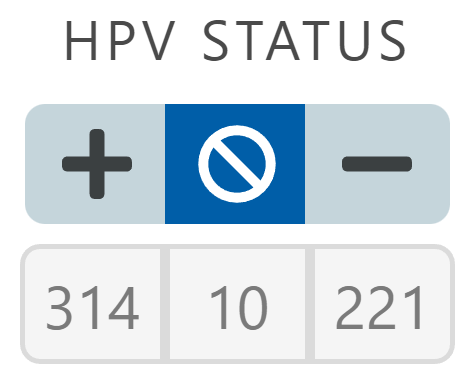
\includegraphics[width=0.18\textwidth]{figures/hpv_neutral.png}
    \end{wrapfigure}
    One such button is shown here on the left. Its switch is in the neutral middle \faIcon{ban} position, as indicated by the highlight in blue, and hence no selection is performed w.r.t. its selection criteria (\gls{hpv} status here). Below the button it shows how many patients in the current selection are \gls{hpv} positive (left number, 314 here), \gls{hpv} negative (right number, 221 here) or do not have \gls{hpv} related information available (number in the middle, 10 here).

    \begin{wrapfigure}{l}{0.2\textwidth}
        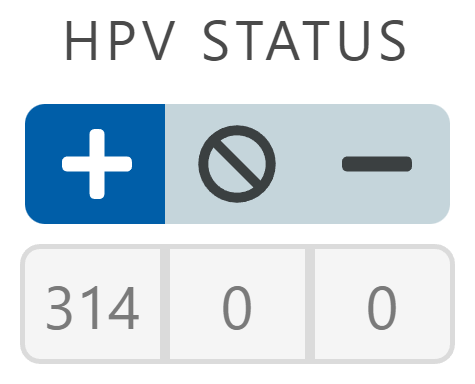
\includegraphics[width=0.18\textwidth]{figures/hpv_positive.png}
    \end{wrapfigure}
    To select all \gls{hpv}-positive patients, a user has to click the \faIcon{plus} symbol. The highlight then switches to the left and after applying the selection (e.g. by clicking the orange ``Compute'' button that appears on the lower right side of the data viewer in \cref{fig:lyprox:data_viewer}) the numbers below the toggle button update as well: Their meaning remains the same, but since the patient selection now only contains \gls{hpv} positive patients, those that are \gls{hpv} negative or have an unknown \gls{hpv} state are filtered out.

    \begin{wrapfigure}{l}{0.2\textwidth}
        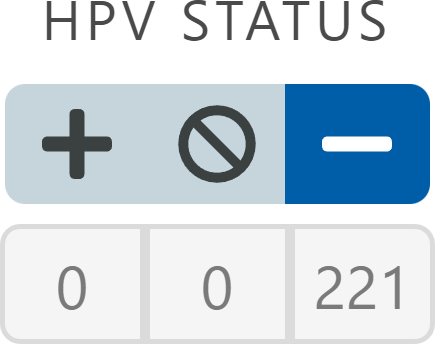
\includegraphics[width=0.18\textwidth]{figures/hpv_negative.png}
    \end{wrapfigure}
    Lastly, to keep only \gls{hpv} negative patients in the selection, the switch has to be brought into the position shown here by clicking the leftmost \faIcon{minus} symbol. Again, after updating/recomputing, the only patients that remain in the selection are the ones whose \gls{hpv} status was reported to be negative.

    
\end{samepage}

As can be seen in \cref{fig:lyprox:data_viewer}, the overall layout  of the interface is divided into five blocks allowing the user to filter patients successively w.r.t. five different aspects:

\begin{itemize}
    \item \textbf{Patient details}~(left column, top box): Four three-way toggle buttons allow patient selection by general information: Whether patients were reported to be smokers, their treatment included a \acrlong{nd}, they were \gls{hpv} positive/negative and whether they were $N_0$ or $N_+$ patients.
    \item \textbf{Primary tumor}~(left column, bottom box): Offers selection criteria related to the tumor. Two toggle buttons allow selection w.r.t. to the lateralization (central/asymmetric and extension over the mid-sagittal plane) and multiple buttons to (de)select patients with tumors originating in various locations and subsites. Lastly in that box, one can (de)select tumors of certain T-categories.
    \item \textbf{Datasets}~(right column, top bar): In this row we list the different datasets and how many patients of each cohort are included in the selection. Here, the user can also (de)select patients from any cohort that they do (not) want to be included.
    \item \textbf{Modalities}~(right column, second bar from top): With the buttons in this bar, users can select patients based on available modalities. E.g., one can select only patients for which pathology reports are available. When different modalities were used to diagnose different patients, selecting multiple modalities here joins the patients that have at least one of modalities and displays the involvement based on what is reported for each patient. Further, if more than one of the selected modalities are available for a patient in the selection, possible conflicts in the involvement reports may be resolved through different methods. For instance, both a \gls{pet} scan and \gls{mri} images could have been taken of a patient's neck and a particular \gls{lnl} may look healthy on the \gls{mri} images, but metastatic on \gls{pet}. Two of the implemented methods to lift these conflicts are the logical \texttt{OR}, displaying an \gls{lnl} as metastatic as soon as one of the available modalities reports involvement, and the maximum likelihood approach introduced in \cref{sec:dataset_clb:methods:max_llh} that uses sensitivity and specificity to establish a consensus.
    \item \textbf{Contra- \& ipsilateral Involvement}~(right column, two large boxes next to each other): The main information is displayed here. Within each box for the corresponding side, we display the prevalence of metastases per \gls{lnl} as observed in the set of patients in the current selection. Every level is shown in its own labelled row that is equipped with another three-way toggle button. Setting it to \faIcon{plus} (and recomputing) causes the interface to only show patients with observed involvement in the respective \gls{lnl}. For example, we can query how many patients show ipsilateral \gls{lnl} IV involvement but a healthy \gls{lnl} V, by setting the button in row ``IV'' of the box to \faIcon{plus}, and in row ``V both'' to \faIcon{minus}. Subsequently, pressing the orange ``compute'' button on the bottom right of the page displays the interface as shown in \cref{fig:lyprox:data_viewer_lnl_example}. To the right of the toggle buttons we plot how many patients in the selected cohort show involvement of the respective \gls{lnl}. It is a horizontally stacked bar plot: The red bar indicates the portion of patients with metastases in the level, the green bar the portion of patients without metastases and a gray bar indicates the portion of patients for whom information on the involvement in the \gls{lnl} is not available.\\
    [3mm]
    \begin{tikzpicture}
        \node (image) at (0,0) {
            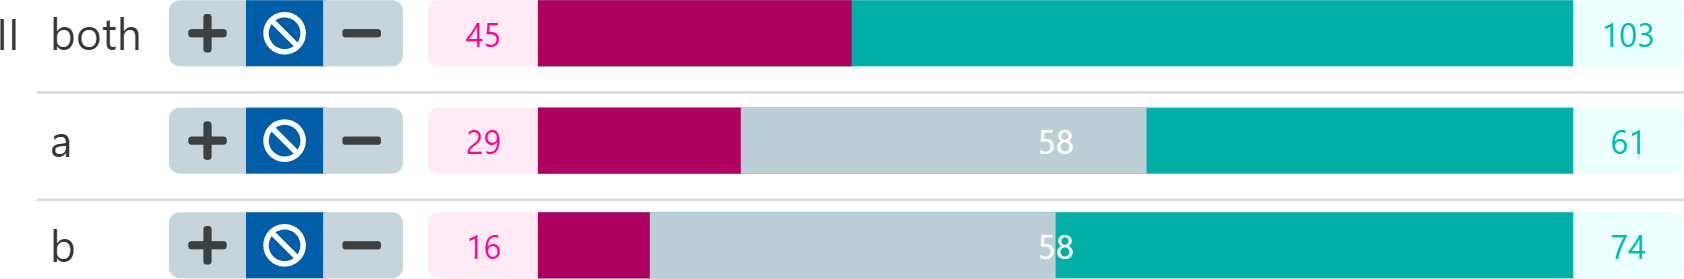
\includegraphics[width=0.92\textwidth]{figures/lnl_bar.png}
        };
        \draw[latex-, very thick, uszorange] (-6.1,1.2) -- (-5.8,1.9) node[above, uszorange]{\small LNL label};
        \draw[latex-, very thick, uszorange] (-4.47,-1.225) -- ++(0.0,-0.5) node[below, uszorange]{\small toggle button};
        \draw[latex-, very thick, uszorange] (-2.7,0.95) edge (-2.0,1.65)
        (-1.5,1.2) -- (-2.0,1.65)
        node[above, uszorange, text width=4.5cm, align=center]{\small number \& portion of patients with involvement};
        \draw[latex-, very thick, uszorange] (3.2,1.2) edge (3.7,1.65)
        (6.05,0.95) -- (3.7,1.65)
        node[above, uszorange, text width=5cm, align=right]{\small number \& portion of patients with a healthy level};
        \draw[latex-, very thick, uszorange] (1.5,-0.2) edge (0.5,-1.725)
        (0.0,-1.2) -- (0.5,-1.725)
        node[below, uszorange, text width=6cm, align=center]{\small number \& portion of patients where LNL status is unknown};
    \end{tikzpicture}\\
    [3mm]
    Above we have labelled the three rows showing the prevalence of involvement in level II contralaterally, along with that \gls{lnl}'s sublevels.
    \item \textbf{Controls}~(right column, bottom bar): In this last box we have placed a few controls: On the left, we have a normal toggle button, allowing the user to switch between percentages and absolute numbers. In case the former is selected, all patient counts in the interface will be replaced by percentages, i.e. absolute numbers divided bz the number of patients in the current selection. On the right we have three buttons (from left to right): The ``\faIcon{question} Help'' button redirects to LyProX' \href{https://lyprox.org/dashboard/help}{\faIcon{external-link-alt}~help page}. The button displaying the total number of patients in selection links to a list of these patients. Finally, the bright orange ``\faIcon{cogs} Compute'' button needs to be pressed for the interface to update, after a user changes the patient selection e.g. via the toggle buttons. We have considered automatically updating the dashboard after each user input, e.g. when a toggle button is switched. However, in that case the number of requests sent to the server would be much larger and the perceived responsiveness of the interface might suffer, because after each click there would be a split-second delay until all numbers and bars update.
\end{itemize}

\begin{figure}
    \centering
    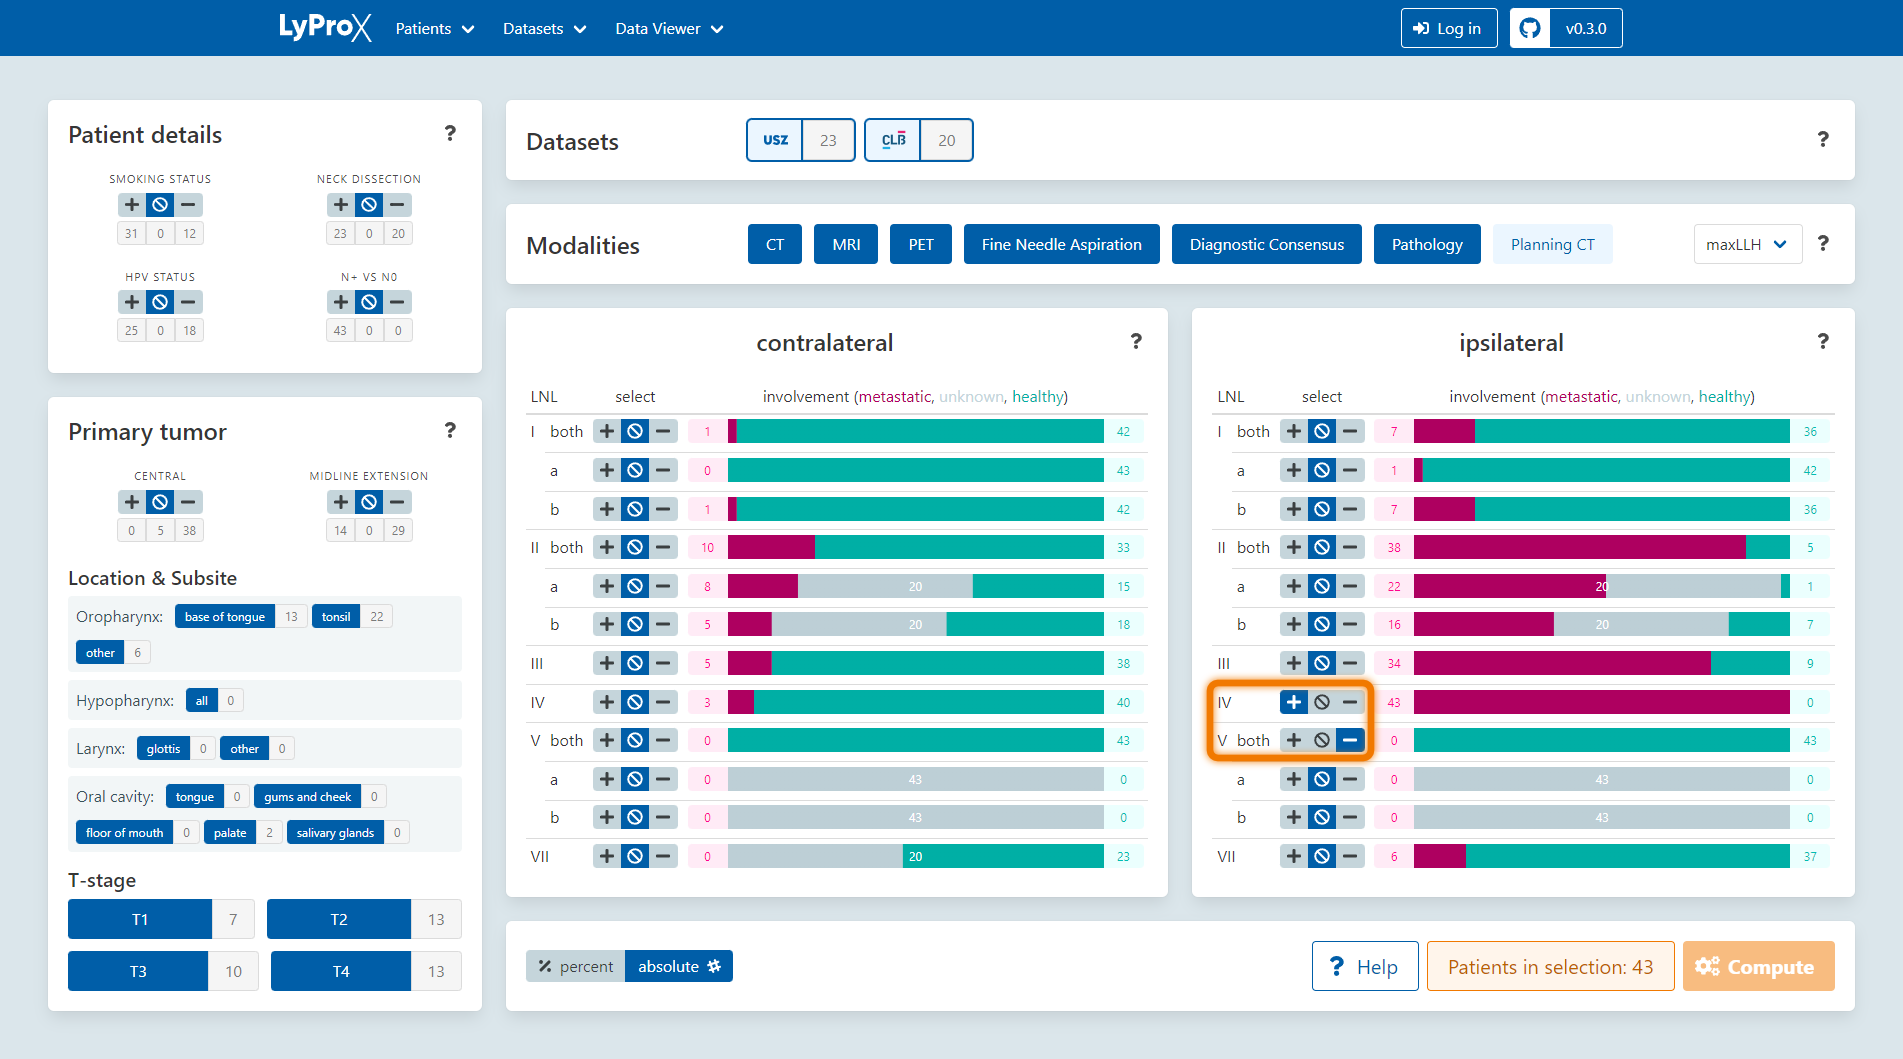
\includegraphics[width=1.0\textwidth, frame]{figures/data_viewer_lnl_example.png}
    \caption[
        The data viewer showing a scenario of two involved LNLs
    ]{
        The data viewer with the following filtering applied: It includes only patients with reported metastases (based on the consensus of selected modalities) in \gls{lnl} IV, without malignancies found in \gls{lnl} V. The three-way toggle buttons whose setting has been changed are outlined in orange.
    }
    \label{fig:lyprox:data_viewer_lnl_example}
\end{figure}

On the mentioned \href{https://lyprox.org/dashboard/help}{\faIcon{external-link-alt}~help page} we have provided an illustrated user manual explaining the concepts and workings of the \gls{gui}. On the same page, one can also find two videos we recorded, showing how to get started with exploring patterns of lymph node involvement using LyProX.

\end{document}
